\documentclass[conference]{IEEEtran}

\usepackage[T1]{fontenc}
\usepackage[utf8]{inputenc}
\usepackage{amsmath,amssymb}
\usepackage{graphicx}
\usepackage{booktabs}
\usepackage{array}
\usepackage{xcolor}
\usepackage{algorithm}
\usepackage{algpseudocode}
\usepackage{pgfplots}
\pgfplotsset{compat=1.18}
\usepackage{pgfplotstable}
\usetikzlibrary{arrows.meta,positioning,shapes.geometric}
\usepackage{cite}
\usepackage{url}
\usepackage{microtype}
\usepackage{balance}

% -----------------------------------------------------------------------
\begin{document}

\title{Reinforcement Learning-Based Adaptive RAW Scheduling\\
       for Dense IEEE 802.11ah IoT Networks}

\author{
  \IEEEauthorblockN{Alakesh Kalita}
  \IEEEauthorblockA{Department of Mathematics and Computing\\
    Indian Institute of Technology (ISM) Dhanbad, India\\
    alakesh.kalita1025@gmail.com}
}

\maketitle

% -----------------------------------------------------------------------
\begin{abstract}
IEEE 802.11ah Restricted Access Window (RAW) scheduling dramatically
reduces MAC-layer collisions in dense IoT deployments, but its performance is
highly sensitive to the choice of group count, slot count, and slot duration.
Static and heuristic policies degrade sharply beyond 300~stations because the
beacon budget forces slots too narrow for reliable collision recovery.
In this paper, we present \textbf{RL-RAW}, a Q-learning RAW policy
for IEEE~802.11ah that addresses this limitation through three mechanisms:
(i)~a learnable phase-partition parameter $P$ controlled by two new
Q-learning actions (\textsc{PhasesInc} / \textsc{PhasesDec}), so the agent
discovers \emph{for any} $N$ when splitting beacons across AID slices
improves the reward — with no hardcoded station-count threshold;
(ii)~an eight-dimensional state that includes MAC retry-rate and phase-count
buckets as explicit delay proxies, enabling the agent to observe both
within-slot contention and inter-beacon waiting pressure; and
(iii)~a six-term reward that jointly penalises collisions, RAW overhead,
retry delay, phase-cycling wait, and slot inadequacy alongside the
primary PDR objective.
All thresholds and hyper-parameters are fully configurable; nothing is
hard-coded.
Each of the five RL architectures is trained with \emph{multi-episode},
convergence-based training: starting from a fresh Q-table/network for each
$(\text{architecture}, N)$ pair, training episodes (120\,s each, disjoint
seeds) continue until the change in PDR between consecutive episodes falls
below $0.01$ for two consecutive checks (minimum 3, maximum 20 episodes).
The resulting 30 trained policies are then evaluated over three held-out
seeds (42, 7, 99) and compared against four baselines — No-RAW, Static RAW,
LACA~\cite{taramit2023laca}, and Chang2019~\cite{chang2019traffic} (a
regression-based traffic-aware grouping scheme) — across
$N \in \{100, 200, 400, 600, 800, 1000\}$.
Multi-episode training fundamentally changes the competitive picture
compared to a single training episode.
At $N=100$, LACA remains dominant (PDR $=1.000$), with trained DQN closest
($0.993$).
From $N=200$ onward, a trained RL variant \emph{exceeds every baseline},
something no architecture achieved with single-episode training: PPO leads
at every density $N \geq 200$ — $0.949$ vs.\ $0.940$ for LACA at $N=200$
($+0.9$\,pp), $0.566$ vs.\ $0.384$ for LACA at $N=400$ ($+18.3$\,pp), $0.417$
vs.\ $0.262$ for static RAW at $N=600$ ($+15.5$\,pp), $0.281$ vs.\ $0.189$ for
static RAW at $N=800$ ($+9.1$\,pp), and $0.210$ vs.\ $0.148$ for static RAW
at $N=1000$ ($+6.3$\,pp).
At $N=100$, PPO is, unusually, the \emph{weakest} RL variant ($0.863$).
Energy efficiency improves correspondingly: Tab-DDQN leads at $N=100$
($61.8$ vs.\ $54.9$ for LACA, $+12.5\,\%$), DDQN leads at $N=200$ ($51.3$
vs.\ $43.3$ for LACA, $+18.6\,\%$), and PPO leads at $N\in\{400,600,800,1000\}$
($34.0$/$24.8$/$15.0$/$10.1$ vs.\ $19.7$/$12.6$/$8.5$/$6.0$ for the best
baseline, i.e.\ $+73$/$+96$/$+76$/$+68\,\%$).
Across a 42-chance win-count tally (7 metrics $\times$ 6 densities),
PPO alone accounts for 28 wins, far ahead of LACA (7), No-RAW (5, mostly
delay artefacts of its near-zero PDR), Tab-DDQN (1), and DDQN (1); tabular
Q-learning, DQN, and static RAW win nothing.
The cost of these PDR/EE gains remains delay: at $N \geq 400$, the best RL
delay is $38$--$176\,\%$ higher than No-RAW's artificially low value, growing
with $N$.
\end{abstract}

\begin{IEEEkeywords}
IEEE 802.11ah, Wi-Fi HaLow, Restricted Access Window, RAW,
reinforcement learning, Q-learning, IoT, dense networks.
\end{IEEEkeywords}

% -----------------------------------------------------------------------
\section{Introduction}

The rapid growth of Internet of Things (IoT) applications has led to the
deployment of networks containing hundreds or even thousands of low-power
devices.
Supporting such a large number of stations (STAs) efficiently is challenging
because simultaneous channel access causes severe contention.
To reduce channel contention, IEEE~802.11ah introduces the Restricted Access
Window (RAW)-based channel access mechanism.
In RAW, the Access Point (AP) divides the beacon interval into access windows
and allows only a selected set of STAs to contend within a particular slot.
The RAW configuration is announced through the RAW Parameter Set (RPS) field
in the beacon frame, so only assigned STAs wake up and contend in their slots,
while the remaining STAs stay in sleep mode~\cite{std80211ah}.

However, RAW performance is strongly dependent on the correct configuration
of group count $G$, per-group slot count $S$, and slot duration $T_\text{slot}$.
If a group contains too many active STAs, collisions and back-off delay
increase.
If too many groups are created, the beacon interval is fragmented into small
windows.
If $T_\text{slot}$ is too small, a STA cannot complete a full DATA–ACK
exchange; if it is too large, beacon time is wasted.
The constraint $G \times S \times T_\text{slot} \leq \eta T_B$ is binding
at high $N$: at $N = 1000$ with $G = 8$, $S = 8$, each slot spans only
$\approx 7\,\text{ms}$, below the physical minimum of $\approx 12\,\text{ms}$
needed for collision recovery at MCS0.

Existing approaches (static, CUSUM-EWMA adaptive, LACA) all allocate
RAW to \emph{all} STAs in every beacon.
Slot duration per STA therefore collapses as $N$ grows, and none of these
schemes explicitly enforces the collision-recovery window.
There is a need for a policy that adapts the complete RAW parameter set
autonomously, without requiring pre-computed tables or explicit STA feedback.
In this paper, we propose \textbf{RL-RAW}, a reinforcement learning approach
that learns optimal RAW parameters end-to-end at the MAC layer.
The main contributions are:
\begin{itemize}
  \item We propose a tabular Q-learning RAW policy with an
        \emph{eight-dimensional} state space and \emph{nine} discrete
        actions, trained end-to-end using only AP-side MAC statistics
        without any STA feedback.  All bucketing thresholds and
        hyper-parameters are configurable — nothing is hard-coded.
  \item We introduce \textsc{PhasesInc} and \textsc{PhasesDec} as two
        new Q-learning actions that let the agent control the AID-space
        partitioning count $P$ directly.  The policy starts at $P = 1$
        for \emph{all} $N$ and learns through the reward signal when
        splitting beacons across AID slices helps — eliminating any
        hardcoded station-count threshold.
  \item We design a \emph{six-term delay-aware reward} that augments the
        PDR, collision, and RAW-overhead terms with MAC retry-rate,
        phase-cycling wait, and slot-adequacy penalties, directly penalising
        configurations that force STAs into repeated back-off or long
        inter-beacon waiting cycles.
  \item We add a \emph{retry-rate bucket} as the seventh state dimension
        and a \emph{phase-count bucket} as the eighth, giving the agent
        distinct signals for within-slot contention delay and inter-beacon
        waiting delay.
  \item We evaluate RL-RAW against three baseline policies
        (No-RAW, Static RAW, and LACA) across
        $N \in \{100, 200, 400, 600, 800, 1000\}$ using a corrected
        implementation with consistent action masking across all selection
        paths and masked Bellman targets, reporting the resulting
        PDR, delay, and energy-efficiency results at each density level.
  \item We implement and train five RL controller architectures —
        tabular Q-learning, tabular Double Q-learning (Tab-DDQN, a
        two-table variant, not a neural network), DQN, Double DQN, and PPO
        — using \emph{multi-episode, convergence-based training} (up to 20
        episodes per architecture/$N$ pair, stopping once consecutive-episode
        PDR change falls below $0.01$).  After training, PPO becomes the
        dominant architecture overall (28 of 42 win-count chances), and PPO
        exceeds every baseline at every $N \geq 200$ — a result not
        achievable with a single training episode.  At $N=100$, PPO is
        instead the weakest RL variant, and LACA remains the best overall
        choice.
\end{itemize}

% -----------------------------------------------------------------------
\section{Related Work}

Several surveys have highlighted IEEE~802.11ah as a key enabler for
large-scale IoT deployments, offering sub-1\,GHz coverage, energy efficiency,
and scalability beyond traditional wireless technologies~\cite{tian2021survey,
ahmed2021mac}.
On the RAW grouping front, TAROA~\cite{tian2016taroa} adapts group assignments
at each beacon based on AP-side traffic estimates, improving throughput in
dense networks; E-TAROA~\cite{tian2017etaroa} refines the estimator for
faster convergence under high density.
RO-RAW~\cite{liu2020roraw} applies an Extended Kalman Filter to estimate
the number of competing stations at runtime and tunes both group count and
slot count accordingly.
Chang et al.~\cite{chang2019traffic} demonstrate through regression analysis
that grouping performance is closely tied to traffic demand heterogeneity and
propose a traffic-proportional grouping design.
Hasi et al.~\cite{hasi2022} extend runtime adaptation by incorporating
predicted demand to enforce load balance across heterogeneous groups.
On the slot-sizing side, Taramit et al.~\cite{taramit2023laca} propose a
load-aware renewal-process model for RAW slot duration, but restrict
evaluation to a single fixed group.
The Neuro-Fuzzy ARX approach of~\cite{nandhini2025} combines an ARX predictor
with an ANFIS decision layer to adapt RAW duration in event-triggered networks,
but the inference complexity is impractical for resource-constrained boards.

All of these works treat RAW group formation and slot sizing as separate
problems, calibrated for specific traffic assumptions.
None learns the full parameter set from experience.
Reinforcement learning has been applied to wireless MAC scheduling in other
contexts~\cite{mnih2015,sutton2018}, but Q-learning for IEEE~802.11ah RAW
is unexplored.
RL-RAW fills this gap by jointly learning $G$, $S$, and $T_\text{slot}$
from the AP's own receive statistics, adapting continuously to the observed
network state.

% -----------------------------------------------------------------------
\section{System Model}

We consider a single-cell IEEE~802.11ah network with one AP and $N$ uplink
STAs.
The AP broadcasts a DTIM beacon every $T_B$ seconds.
Each beacon carries the RPS, through which the AP assigns STAs to $G$
contiguous RAW groups with per-group slot count $S$ and slot duration
$T_\text{slot}$.
Let the associated STAs be represented by their AIDs $\{1, \ldots, N\}$.

A STA may contend for the channel only during its assigned RAW slot;
otherwise it remains in sleep mode.
The complete RAW schedule must satisfy the beacon-budget constraint:
\begin{equation}
  G \times S \times T_\text{slot} \leq \eta T_B,
  \label{eq:budget}
\end{equation}
where $\eta = 0.9$ reserves 10\,\% of the beacon interval for overhead.

For a successful DATA–ACK exchange to occur within a slot, the slot must
accommodate at least one complete exchange sequence.
At MCS0 (150\,kbps) with a 128-byte payload and 14-byte ACK, this physical
minimum is:
\begin{equation}
  T_\text{min} = t_\text{data} + t_\text{SIFS} + t_\text{ACK} +
                 t_\text{DIFS} + \bar{t}_\text{bo} + t_\text{guard}
                 \approx 12\,\text{ms},
  \label{eq:tmin}
\end{equation}
where $\bar{t}_\text{bo} = \frac{W_0 - 1}{2} \sigma$ is the average
back-off with minimum contention window $W_0 = 16$ and slot time
$\sigma = 52\,\mu\text{s}$.
Any slot shorter than $T_\text{min}$ is very unlikely to deliver a packet
reliably, since it cannot accommodate a complete DATA–ACK exchange
plus typical back-off time.

The AP observes four cumulative MAC statistics at each beacon boundary,
computed as deltas from the previous beacon:
$\Delta_\text{rx}$ (successful uplink receptions),
$\Delta_\text{err}$ (CRC errors),
$\Delta_\text{tx}$ (total transmission attempts), and
$\Delta_\text{rtr}$ (MAC retries).
The RL policy uses only these AP-side observations and requires no
queue-status reports or explicit STA feedback.
The retry rate $\rho = \Delta_\text{rtr}/\Delta_\text{tx} \in [0,1]$
serves as a MAC-layer delay proxy: high retries indicate repeated back-off
cycles and elevated queuing delay.

% -----------------------------------------------------------------------
\section{Proposed RL-RAW Scheme}

At each beacon boundary, the RL-RAW agent observes the current network
state, receives a reward reflecting the outcome of the previous configuration,
updates the Q-table, and selects the next RAW parameters.
Fig.~\ref{fig:rl_loop} illustrates the closed-loop interaction.

\begin{figure}[t]
\centering
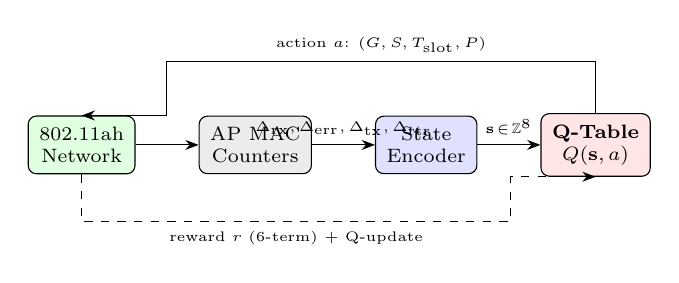
\begin{tikzpicture}[
  >=Stealth, node distance=0.55cm, font=\scriptsize,
  B/.style={draw, rounded corners=3pt, fill=#1,
            minimum height=0.72cm, align=center, inner sep=4pt},
]
\node[B=green!12] (net)
      {802.11ah\\Network};
\node[B=gray!15, right=0.8cm of net] (obs)
      {AP MAC\\Counters};
\node[B=blue!12, right=0.8cm of obs] (enc)
      {State\\Encoder};
\node[B=red!10,  right=0.8cm of enc] (agt)
      {\textbf{Q-Table}\\$Q(\mathbf{s},a)$};

\draw[->] (net) -- (obs);
\draw[->] (obs) -- node[above]{\tiny$\Delta_\text{rx},\Delta_\text{err},\Delta_\text{tx},\Delta_\text{rtr}$} (enc);
\draw[->] (enc) -- node[above]{\tiny$\mathbf{s}\!\in\!\mathbb{Z}^8$} (agt);

% action arrow arching above
\draw[->] (agt.north) -- ++(0,0.65)
    -- node[above, align=center]{\tiny action $a$: $(G,S,T_\text{slot},P)$}
    ++(-5.45,0) |- (net.north);

% reward arrow arching below (dashed)
\draw[->, dashed] (net.south) -- ++(0,-0.60)
    -- node[below]{\tiny reward $r$ (6-term) + Q-update}
    ++(5.45,0) |- (agt.south);

\end{tikzpicture}
\caption{RL-RAW per-beacon control loop. The four AP MAC counters are
  bucketed into an 8-dimensional state $\mathbf{s}$; the Q-table selects one
  of 9 actions that updates $(G,S,T_\text{slot},P)$ subject to the beacon
  budget; and the 6-term reward drives the Q-table update via experience
  replay.}
\label{fig:rl_loop}
\end{figure}

\subsection{State Space}

The agent observes an \textbf{eight-dimensional} discrete state
$\mathbf{s} = (b_c, b_p, b_n, i_G, b_s, b_\delta, b_r, b_P)$
at each beacon boundary.
Table~\ref{tab:state} summarises all eight dimensions; all bucketing
thresholds are configurable.

\begin{table}[h]
\centering
\caption{Eight-Dimensional State Space of RL-RAW}
\label{tab:state}
\setlength{\tabcolsep}{3pt}
{\scriptsize
\begin{tabular}{clcll}
\toprule
Dim & Symbol & Range & Formula / Source & Captures \\
\midrule
1 & $b_c$ & $\{0,1,2\}$
  & $c=\frac{\Delta_\text{err}}{\Delta_\text{rx}+\Delta_\text{err}}$;
    thr.\ 10\%,30\%
  & Collision level \\[3pt]
2 & $b_p$ & $\{0,1,2\}$
  & $\hat{p}=\frac{\Delta_\text{rx}}{n_\phi\,\tau}$; thr.\ 60\%,30\%
    ($b_p{=}0$: $\geq$60\% good; $b_p{=}1$: 30–60\%; $b_p{=}2$: $<$30\% poor)
  & PDR level \\[3pt]
3 & $b_n$ & $\{0,1,2,3\}$
  & $N=n_\phi P$; thr.\ 100,300,600
  & Network density \\[3pt]
4 & $i_G$ & $\{0,1,2,3\}$
  & index into $\mathcal{G}=\{1,2,4,8\}$
  & Current group count \\[3pt]
5 & $b_s$ & $\{0,1,2\}$
  & normalised $T_\text{slot}$; thr.\ 33\%,67\%
  & Slot width \\[3pt]
6 & $b_\delta$ & $\{0,1\}$
  & 1 if $\hat{p}<\mathrm{EMA}(\hat{p})$
  & PDR trend (falling?) \\[3pt]
7 & $b_r$ & $\{0,1,2\}$
  & $\rho_r=\frac{\Delta_\text{rtr}}{\Delta_\text{tx}}$;
    thr.\ 30\%,60\%
  & Within-slot contention delay \\[3pt]
8 & $b_P$ & $\{0,1,2\}$
  & $P$; thr.\ 2, 4
  & Inter-beacon wait (phases) \\
\bottomrule
\end{tabular}
}
\end{table}

The PDR bucket $b_p$ is encoded ascending: $b_p=0$ denotes good PDR
($\hat{p}\geq60\,\%$), $b_p=1$ moderate ($30\text{--}60\,\%$), and
$b_p=2$ poor ($<30\,\%$).
Dimensions 7--8 are new contributions of this work.
$b_r$ captures within-slot back-off pressure (higher $b_r$ = more retries
= more contention); $b_P$ captures inter-beacon scheduling delay from phase
cycling.
Together they let Q-learning assign credit correctly: G/S/slot actions own
$b_r$, while \textsc{PhasesInc}/\textsc{PhasesDec} own $b_P$.
$b_P = 0$ means $P=1$ (no phase wait); $b_P = 1$ means $P\in\{2,3\}$
(moderate wait); $b_P = 2$ means $P\geq 4$ (significant wait).

The total state space is
$3\!\times\!3\!\times\!4\!\times\!4\!\times\!3\!\times\!2\!\times\!3\!\times\!3 = 7776$
states; in practice fewer than 200 are visited per $N$ value, confirming
tractability for tabular Q-learning.
Unseen states are initialised with context-sensitive priors:
$Q(\mathbf{s},\textsc{Keep}) = \kappa$ supplemented by physics-motivated biases
(e.g.\ $Q(\mathbf{s},\textsc{PhasesInc}) \mathrel{+}= \beta$ when
$b_r = 2$ and $b_P = 0$), both configurable.

\subsection{Learnable Phase Partitioning}

The AID space may be divided into $P$ equal slices so that each beacon
activates RAW for exactly one slice in round-robin order.
When $P > 1$, only $\lfloor N/P \rfloor$ STAs contend per beacon, widening
each slot and reducing per-slot collision probability.
The cost is delay: each STA waits up to $P \cdot T_B$ seconds between RAW
opportunities, which is captured by the phase-count bucket $b_P$ and
penalised through the $-w_\phi\phi$ term in the reward
(not through the retry-rate bucket $b_r$, which is owned by G/S/slot actions).

\textbf{Key design}: $P$ is a \emph{Q-learning parameter}, not a function of
$N$.  The policy always starts at $P = 1$ regardless of station count.
Two new actions let Q-learning adjust it at every beacon:
\begin{itemize}
  \item \textsc{PhasesInc} — increase $P$ by 1 (serve fewer STAs, wider slots)
  \item \textsc{PhasesDec} — decrease $P$ by 1 (serve more STAs, less delay)
\end{itemize}
The only constraint on $P$ is derived from traffic timing, not from $N$:
\begin{equation}
  1 \leq P \leq P_\text{max} = \left\lfloor \frac{T_\text{traffic}}{T_B}
  \right\rfloor,
  \label{eq:phases}
\end{equation}
which guarantees every STA receives at least one RAW opportunity per packet
interval.  For $T_\text{traffic} = 5\,\text{s}$, $T_B = 0.5\,\text{s}$,
$P_\text{max} = 10$.

Q-learning discovers the right $P$ through the reward signal: at high $N$,
$P = 1$ produces narrow slots, high collisions, and high retry rates — all
penalised.  The agent learns \textsc{PhasesInc} relieves this, while
\textsc{PhasesDec} is rewarded when the network is lightly loaded and delay
can be reduced without harming PDR.
This eliminates any hardcoded station-count threshold from the policy.

\subsection{Reward Function}

After each beacon interval, the agent receives a \textbf{six-term} reward:
\begin{equation}
  r = w_p \hat{p} - w_c c - w_h h
      - w_r \rho_r - w_\phi \phi - w_s \sigma,
  \label{eq:reward}
\end{equation}
where $\hat{p}$ is the per-phase PDR normalised to the previous phase size;
$c = \Delta_\text{err}/(\Delta_\text{rx}+\Delta_\text{err})$ is the collision
fraction; $h = G S T_\text{slot}/(0.9\,T_B)$ is the normalised RAW overhead;
$\rho_r = \Delta_\text{rtr}/\Delta_\text{tx}$ is the MAC retry rate;
$\phi = \min(1,\,(P-1)\,T_B/T_\text{traffic})$ is the normalised
phase-cycling wait; and
$\sigma = \max(0,\,1 - T_\text{slot}/T_\text{min})$ is the slot-adequacy
deficit.
All six weights are configurable; defaults are
$(w_p, w_c, w_h, w_r, w_\phi, w_s) = (1.0, 0.4, 0.1, 0.3, 0.5, 0.3)$.

The critical addition in v8 is the phase-cycling term $-w_\phi \phi$.
Prior to v8, delay was penalised only through $\rho_r$ (MAC retries), which
is influenced by G, S, and $T_\text{slot}$ but is \emph{insensitive to $P$}.
The $\phi$ term is directly zero when $P = 1$ and grows as $P$ increases,
giving Q-learning an explicit signal to prefer smaller $P$ when PDR can be
maintained without additional phases.
The two delay terms are deliberately separate: $\rho_r$ is owned by
G/S/slot actions, while $\phi$ is owned exclusively by the
\textsc{PhasesInc}/\textsc{PhasesDec} actions, enabling correct credit
assignment.

The denominator of $\hat{p}$ uses the phase STA count at the \emph{previous}
beacon, correctly attributing the reward to the configuration that was active
during the measured interval.

\subsection{Q-Learning Update}

Algorithm~\ref{alg:rl} details the per-beacon procedure.
The TD target applies the standard Q-learning Bellman backup~\cite{watkins1992}
with configurable clipping to $[-C, C]$ (default $C = 5$) for stability:
\begin{equation}
  \delta = r + \gamma \max_{a' \in \mathcal{A}_\text{valid}(\mathbf{s}')} Q(\mathbf{s}', a') - Q(\mathbf{s}, a),
  \label{eq:td}
\end{equation}
\begin{equation}
  Q(\mathbf{s}, a) \leftarrow Q(\mathbf{s}, a) + \alpha\,\text{clip}(\delta, -C, C).
  \label{eq:qupdate}
\end{equation}
An experience replay buffer (capacity 200, batch size 16, up to 5 replay
updates per step) is maintained to decorrelate consecutive transitions.
Both the primary Q-update and replay pushes are guarded by
$\Delta_\text{rx}>0$ or $\Delta_\text{err}>0$: beacons with no observable
traffic produce no learning signal so idle-beacon noise is never
injected into the Q-table.
The Bellman max/argmax over the \emph{next} state is computed only over
valid actions (those not excluded by the action mask for $\mathbf{s}'$),
so Q-values for forbidden actions cannot inflate the bootstrap target.
The same mask is applied to both exploration and greedy selection.
Epsilon decay is suspended during the 5-beacon cold-start phase so that
$\varepsilon$ does not decay before any Q-values are populated.
After cold-start, $\varepsilon$ decays as
$\varepsilon \leftarrow \max(\varepsilon_\text{min},\, \varepsilon \cdot d_\varepsilon)$
(defaults: $d_\varepsilon = 0.985$, $\varepsilon_\text{min} = 0.05$).

The action space contains nine discrete actions summarised in
Table~\ref{tab:actions}.
Actions 2--7 tune the three RAW parameters $(G,S,T_\text{slot})$;
actions 8--9 adjust the phase count $P$, a capability unique to RL-RAW.
All budget constraints (Eq.~(\ref{eq:budget})) are enforced after applying
the chosen action.

\begin{table}[h]
\centering
\caption{Action Space: Nine Discrete Actions}
\label{tab:actions}
{\scriptsize
\begin{tabular}{clll}
\toprule
\# & Action & Effect & Constraint / Mask \\
\midrule
1 & \textsc{Keep}       & No change                                   & — \\
2 & \textsc{SlotInc}    & $T_\text{slot} \mathrel{+}= \Delta_T$       & Eq.~(\ref{eq:budget}) \\
3 & \textsc{SlotDec}    & $T_\text{slot} \mathrel{-}= \Delta_T$       & $T_\text{slot}\geq T_\text{min}$ \\
4 & \textsc{GroupsInc}  & $G\leftarrow\text{next in }\mathcal{G}$     & Eq.~(\ref{eq:budget}) \\
5 & \textsc{GroupsDec}  & $G\leftarrow\text{prev in }\mathcal{G}$     & $G\geq 1$; masked if $b_p=2$ (poor PDR) \\
6 & \textsc{NSlotsInc}  & $S \mathrel{+}= 1$                          & Eq.~(\ref{eq:budget}) \\
7 & \textsc{NSlotsDec}  & $S \mathrel{-}= 1$                          & $S\geq 1$; never random-explored \\
8 & \textsc{PhasesInc}  & $P \mathrel{+}= 1$                          & $P\leq P_\text{max}$; masked if $b_P\!\geq\!1$ and $b_p\!=\!0$ \\
9 & \textsc{PhasesDec}  & $P \mathrel{-}= 1$                          & $P\geq 1$; masked if $b_r>0$ \\
\bottomrule
\end{tabular}
}
\end{table}

The masks are derived from state, not station count:
The masks prevent harmful random exploration but do \emph{not} restrict
the greedy path, which may select any of the nine actions:
\textsc{NSlotsDec} is never explored randomly because decreasing $S$
silently worsens per-slot contention;
\textsc{PhasesDec} is excluded from random exploration when $b_r > 0$
(elevated retries signal that reducing phases would worsen inter-beacon
delay);
\textsc{PhasesInc} is excluded when $b_P\!\geq\!1$ and $b_p\!=\!0$
(phases are already elevated and PDR is already good — adding more delay is
counter-productive);
\textsc{GroupsDec} and \textsc{SlotDec} are excluded when $b_p = 2$
(PDR already poor — reducing groups or slot width increases per-group
contention and makes recovery harder).

\begin{algorithm}[t]
\caption{RL-RAW v8: per-beacon Q-learning update}
\label{alg:rl}
\begin{algorithmic}[1]
\Require Current state $\mathbf{s}$, buffer $\mathcal{B}$,
         params $\alpha, \gamma, \varepsilon, C$;
         $\mathbf{s}_-=\mathtt{None}$, $a_-=\mathtt{None}$ at first beacon
\State Observe $\Delta_\text{rx}, \Delta_\text{err}, \Delta_\text{tx},
       \Delta_\text{rtr}$ from AP MAC stats
\State Compute 6-term reward $r$ using~(\ref{eq:reward})
\If{$\mathbf{s}_- \neq \mathtt{None}$ \textbf{and} not cold-start}
  \If{traffic detected ($\Delta_\text{rx} > 0$ \textbf{or} $\Delta_\text{err} > 0$)}
    \State Push $(\mathbf{s}_-, a_-, r, \mathbf{s})$ to $\mathcal{B}$
  \EndIf
  \State $\delta \gets r + \gamma \max_{a'} Q(\mathbf{s}, a') - Q(\mathbf{s}_-, a_-)$
  \State $Q(\mathbf{s}_-, a_-) \mathrel{+}= \alpha \cdot \text{clip}(\delta, -C, C)$
  \For{$k = 1$ \textbf{to} $\min(U, |\mathcal{B}|/B)$}
    \State Sample mini-batch from $\mathcal{B}$; apply TD update for each
  \EndFor
\EndIf
\State $a \leftarrow \textsc{Select}(\mathbf{s}, \varepsilon)$
       \Comment{9 actions, uniform across all $N$}
\State Apply $a$ (including $P \mathrel{+}= 1$ / $P \mathrel{-}= 1$);
       enforce budget~(\ref{eq:budget})
\State $(\mathbf{s}_-, a_-) \leftarrow (\mathbf{s}, a)$
\If{not cold-start}
  \State $\varepsilon \leftarrow \max(\varepsilon_\text{min},\, \varepsilon \cdot d_\varepsilon)$
\EndIf
\end{algorithmic}
\end{algorithm}

The Q-table, visit counts, and $\varepsilon$ are persisted to disk after each
120-second episode, enabling multi-episode training across disjoint seeds.
At evaluation time, $\varepsilon = 0.02$ is used for near-greedy exploitation.

\subsection{Supported RL Controller Architectures}

All five architectures share the same 8-dimensional state space, 6-term
reward, 9-action set, and phase-partitioning mechanism; they differ only in
the update rule and exploration strategy.
Four are value-based (tabular Q-learning, Tab-DDQN, DQN, DDQN — where
tabular Q-learning and Tab-DDQN use Python dictionaries and DQN/DDQN use
two-layer ReLU networks); one is a policy-gradient actor-critic method (PPO).
All five architectures apply the same action mask to \emph{every} selection
path — exploration, UCB, and greedy — so forbidden actions are never executed
regardless of the selection mode.

\textbf{Tabular Q-learning} (primary proposal) stores $Q(\mathbf{s},a)$
in a Python dictionary and applies~(\ref{eq:qupdate}) directly.
It is the most memory-efficient and fastest-converging option.

\textbf{Double tabular Q-learning} (Tab-DDQN; \emph{not} a neural-network
variant) maintains two dictionary-based Q-tables $Q_1, Q_2$~\cite{hasselt2010}.
At each step one table is chosen at random to be updated; the other evaluates
$Q(s',\arg\max_{a'}Q_\text{update}(s',a'))$, eliminating the maximisation
bias of vanilla Q-learning.
The greedy action averages both tables.
Tab-DDQN shares no neural-network components with DDQN.

\textbf{DQN} replaces the Q-table with a two-layer ReLU network
(He init, configurable hidden size $h$) implemented in pure NumPy.
A single MSE gradient step is taken per sample; the same experience-replay
buffer is shared with tabular modes~\cite{mnih2015}.

\textbf{Double DQN (DDQN)} decouples action selection (online network)
from value evaluation (periodically hard-copied target network), reducing
overestimation in the Bellman target~\cite{vanhasselt2016}.
The target network is updated every \texttt{target\_update\_freq} steps
(default 20).

\textbf{PPO} maintains separate actor ($\pi_\theta$, softmax output) and
critic ($V_\phi$, scalar output) networks.
Transitions are collected into a fixed-length on-policy rollout buffer
(default 16 steps); advantages are computed via Generalised Advantage
Estimation ($\lambda_\text{GAE}=0.95$)~\cite{schulman2015} and the
actor is trained with the clipped surrogate objective
$L_\text{clip}=-\min\!\left(r_t A_t,\,
\text{clip}(r_t,1\!-\!\varepsilon_c,1\!+\!\varepsilon_c)\,A_t\right)$
plus an entropy bonus.
Exploration is stochastic (policy distribution), with the same action
masks applied before sampling.
The boolean mask used at sampling time is stored in the rollout buffer
so that the importance-sampling ratio
$\rho_t = \pi_\theta(a_t|s_t,m_t)/\pi_{\theta_\text{old}}(a_t|s_t,m_t)$
is computed under the same constrained distribution for both old and new
log-probabilities.
$\varepsilon$-decay is disabled for PPO.

% -----------------------------------------------------------------------
\section{Performance Evaluation}

\subsection{Simulation Setup}
\label{sec:setup}

We implement RL-RAW in our own Python-based IEEE~802.11ah simulator\footnote{
\url{https://github.com/alakesh-kalita/sim11ah}}.
Results are averaged over three independent seeds (42, 7, and 99), and error
bars represent 95\,\% confidence intervals.
Table~\ref{tab:params} summarises the simulation parameters.
Four baselines are evaluated: \textbf{No-RAW} (unrestricted DCF);
\textbf{Static RAW} (fixed $G=1$, $S=8$, $T_\text{slot}=14\,\text{ms}$);
\textbf{LACA}~\cite{taramit2023laca} (load-aware renewal-process slot sizing);
and \textbf{Chang2019}~\cite{chang2019traffic} (regression-based
traffic-aware sensor grouping, re-implemented with a greedy max-min-fairness
boundary-rebalancing scheme adapted to AID-contiguous RAW groups and the
same Bianchi/LACA renewal-process slot sizing as LACA).

\textbf{Multi-episode training.}
Each of the five RL architectures is trained independently for each
$N \in \{100,\ldots,1000\}$, giving 30 (architecture, $N$) checkpoints.
Training starts from an empty Q-table/network and proceeds in 120\,s
episodes on a fixed sequence of 20 disjoint training seeds, with the
Q-table/network, optimiser state, visit counts, and $\varepsilon$ persisted
to disk after every episode.
Training stops for a given (architecture, $N$) pair once at least 3 episodes
have run \emph{and} the absolute PDR change between the last two consecutive
episode pairs is both below $0.01$ (i.e.\ two consecutive
$|\Delta\text{PDR}|<0.01$ checks), or after 20 episodes, whichever comes
first.
In practice, most (architecture, $N$) pairs either converge within
3--9 episodes or run the full 20-episode budget; PPO at $N=100$ and
Tab-DDQN at $N=600$ converge fastest (3 episodes).
At evaluation time, each trained checkpoint is loaded with
$\varepsilon = 0.02$ (near-greedy exploitation, no further learning) and
evaluated over the three held-out seeds (42, 7, 99) used for the baselines.

\textbf{Association overhead.}
Before data exchange begins, each STA executes the IEEE~802.11 open-system
procedure: (1)~passive beacon scan (7.1\,ms to the first beacon),
(2)~authentication request/response exchange, and
(3)~association request/response exchange.
Because all $N$ STAs contend for the AP simultaneously and without RAW
protection, the auth and assoc exchanges suffer heavy queuing delay.
Table~\ref{tab:assoc} reports the mean association time per STA from
simulation.
For RAW-enabled policies at $N=200$, the association procedure takes
3.2–3.6\,s (Static: 3.2\,s; LACA: 3.4\,s; RL-RAW: 3.6\,s),
yielding an idle-phase energy contribution of
$P_\text{idle}\times T_\text{assoc}\approx 64$–$72$\,mJ per STA.
No-RAW takes 10.7\,s at $N=200$ ($\approx215$\,mJ/STA) and, at $N\!\geq\!600$,
fails to associate all STAs within the 120\,s window
(success fractions: 81.8\,\% at $N=600$, 60.3\,\% at $N=800$,
48.5\,\% at $N=1000$), further compounding its PDR collapse.
All reported energy totals include the association-phase idle overhead.
The high \emph{observed} MAC retry rate ($\approx35$–$47$\%) is dominated
by management-frame collisions during this association burst; data-phase
retries are fewer than 0.8\,\% of data TX attempts at $N=200$.

\begin{table}[t]
\centering
\caption{Simulation Parameters}
\label{tab:params}
\begin{tabular}{ll}
\toprule
Parameter & Value \\
\midrule
Simulation time          & 120\,s \\
Station counts $N$       & 100, 200, 400, 600, 800, 1000 \\
Traffic model            & Periodic, $T_\text{pkt} = 5\,\text{s/STA}$ \\
Packet payload           & 128\,B \\
PHY mode                 & MCS0 (150\,kb/s, BPSK 1/2) \\
Carrier frequency        & 915\,MHz \\
Propagation delay        & 300\,\textmu{}s \\
Beacon interval $T_B$    & 500\,ms \\
Static slot duration     & 14\,ms \\
RL: $(\alpha, \gamma, \varepsilon_0, \varepsilon_\text{min}, d_\varepsilon)$ & (0.20, 0.90, 0.40, 0.05, 0.985) \\
RL: $(w_p, w_c, w_h, w_r, w_\phi, w_s)$ & (1.0, 0.4, 0.1, 0.3, 0.5, 0.3) \\
RL: initial phases $P_0$ & 1 (learned by Q-learning) \\
RL: max phases $P_\text{max} = \lfloor T_\text{pkt}/T_B \rfloor$ & 10 \\
Seeds                    & 42, 7, 99 \\
\bottomrule
\end{tabular}
\end{table}

\begin{table}[t]
\centering
\caption{Mean Association Time per STA (seconds, mean over 3 seeds).
  RAW policies scale from $\approx$1.5–1.7\,s at $N=100$ to
  $\approx$19–23\,s at $N=1000$; No-RAW fails to associate all STAs
  within 120\,s at $N\!\geq\!600$ (marked $^*$).}
\label{tab:assoc}
\setlength{\tabcolsep}{3pt}
{\scriptsize
\begin{tabular}{r cccc}
\toprule
$N$ & No-RAW & Static & LACA & RL-RAW \\
\midrule
 100 &  2.8        & 1.5 & 1.6 & 1.6 \\
 200 & 10.7        & 3.2 & 3.4 & 3.6 \\
 400 & 32.7        & 7.5 & 7.3 & 7.2 \\
 600 & 47.7$^*$   & 12.1 & 11.2 & 11.5 \\
 800 & 49.4$^*$   & 16.0 & 15.2 & 15.1 \\
1000 & 51.2$^*$   & 20.1 & 19.4 & 18.8 \\
\bottomrule
\end{tabular}
}
\end{table}

\subsection{Packet Delivery Ratio}

Fig.~\ref{fig:pdr} shows the PDR for all nine policies (four baselines,
five multi-episode-trained RL variants), evaluated with the corrected
implementation described in Sec.~\ref{sec:rl}.
At $N = 100$, LACA and Chang2019 both reach a PDR of 1.000 — Chang2019's
regression-based grouping converges to a near-optimal AID partition at this
low contention level, also tying LACA for the highest throughput
(20.48\,kb/s) and fairness ($1.000$) at this density — ahead of every RL
variant; the closest RL controllers are DQN (0.993), tabular Q-learning
(0.989), and Tab-DDQN (0.988), with DDQN (0.969) next, and PPO (0.863)
trailing well behind — the only density at which PPO underperforms every
other RL variant.
This is the only density at which no RL variant surpasses the best baseline.
Chang2019's advantage is short-lived: its PDR collapses to 0.434 at
$N = 200$ and continues falling to 0.188, 0.118, 0.083, and 0.065 at
$N\in\{400,600,800,1000\}$, settling close to Static RAW/No-RAW for
$N\geq400$ rather than tracking LACA — the regression-based grouping and
greedy boundary rebalancing cannot keep pace with the growing per-group
demand imbalance at high station counts.

From $N = 200$ onward, PPO exceeds \emph{every} baseline at \emph{every}
density — a qualitative change from single-episode training, where LACA
remained ahead through $N=200$.
At $N = 200$, PPO reaches 0.949, exceeding LACA (0.940, $+0.9$\,pp,
$+0.9\,\%$); DQN (0.937) and Tab-DDQN (0.921) also approach LACA, with
tabular Q-learning (0.904) close behind, while DDQN (0.846) trails.
At $N = 400$, all five RL variants exceed both LACA (0.384) and static RAW
(0.366); PPO leads (0.566, $+18.3$\,pp over LACA, $+47.6\,\%$), followed by
Tab-DDQN (0.511), DDQN (0.496), tabular (0.479), and DQN (0.458).
At $N = 600$, the best baseline is now static RAW (0.262); PPO leads
(0.417, $+15.5$\,pp, $+59.0\,\%$), with DDQN (0.340) and DQN (0.337)
close behind, and tabular (0.323) and Tab-DDQN (0.296) also exceeding static
RAW.
At $N = 800$, PPO leads (0.281, $+9.1$\,pp over static RAW's 0.189,
$+48.1\,\%$), with tabular (0.251) next; all five RL
variants again exceed static RAW.
At $N = 1000$, PPO leads (0.210, $+6.3$\,pp over static RAW's 0.148,
$+42.5\,\%$), with DDQN (0.196) close behind, and all
five RL variants exceed static RAW.
Overall, PPO is the strongest RL controller at every density except
$N=100$ (where DQN leads among RL variants but still trails LACA) — and at
every $N \geq 200$, PPO beats the best baseline, with margins ranging from
$+0.9$\,pp ($N=200$) to $+18.3$\,pp ($N=400$).

\begin{figure}[t]
\centering
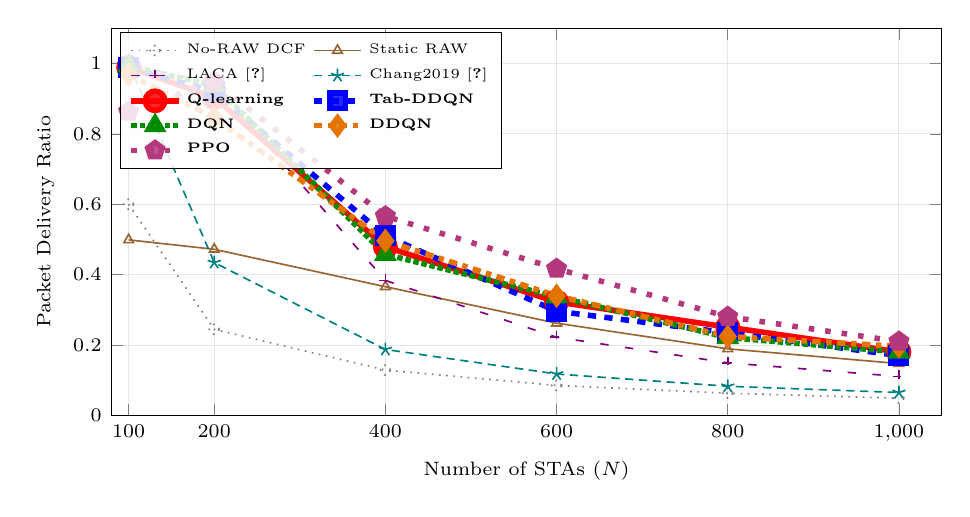
\begin{tikzpicture}
\begin{axis}[
  width=\columnwidth, height=6.5cm,
  xlabel={Number of STAs ($N$)},
  ylabel={Packet Delivery Ratio},
  xmin=80, xmax=1050,
  ymin=0, ymax=1.10,
  xtick={100,200,400,600,800,1000},
  ytick={0,0.2,0.4,0.6,0.8,1.0},
  legend style={font=\tiny, cells={anchor=west}, legend columns=2,
                at={(0.01,0.99)}, anchor=north west, draw=black,
                fill=white, fill opacity=0.85, text opacity=1},
  grid=both, grid style={gray!20},
  tick label style={font=\scriptsize},
  label style={font=\scriptsize},
]
% ---- Baselines: line width=0.6pt, open markers -------------------------
\addplot[color=gray,        line width=0.6pt, dotted,
         mark=o,        mark size=1.8pt] coordinates {
  (100,0.6001)(200,0.2447)(400,0.1290)(600,0.0854)(800,0.0633)(1000,0.0492)
}; \addlegendentry{No-RAW DCF}
\addplot[color=brown!80!black, line width=0.6pt, solid,
         mark=triangle, mark size=2pt] coordinates {
  (100,0.4989)(200,0.4721)(400,0.3658)(600,0.2623)(800,0.1894)(1000,0.1475)
}; \addlegendentry{Static RAW}
\addplot[color=violet,      line width=0.6pt, loosely dashed,
         mark=+,        mark size=2.2pt] coordinates {
  (100,1.0000)(200,0.9398)(400,0.3835)(600,0.2224)(800,0.1497)(1000,0.1109)
}; \addlegendentry{LACA~\cite{taramit2023laca}}
\addplot[color=teal,        line width=0.6pt, densely dashed,
         mark=star,     mark size=2.5pt] coordinates {
  (100,1.0000)(200,0.4344)(400,0.1876)(600,0.1179)(800,0.0831)(1000,0.0653)
}; \addlegendentry{Chang2019~\cite{chang2019traffic}}
% ---- RL variants: line width=2pt, filled markers, each unique style ----
\addplot[color=red,                   line width=2pt,   solid,
         mark=*,        mark size=3.5pt,
         mark options={solid,fill=red}] coordinates {
  (100,0.9890)(200,0.9035)(400,0.4791)(600,0.3226)(800,0.2511)(1000,0.1807)
}; \addlegendentry{\textbf{Q-learning}}
\addplot[color=blue,                  line width=2pt,   dashed,
         mark=square*,  mark size=2.8pt,
         mark options={solid,fill=blue}] coordinates {
  (100,0.9878)(200,0.9209)(400,0.5105)(600,0.2962)(800,0.2349)(1000,0.1701)
}; \addlegendentry{\textbf{Tab-DDQN}}
\addplot[color=green!55!black,        line width=2pt,   densely dotted,
         mark=triangle*, mark size=2.8pt,
         mark options={solid,fill=green!55!black}] coordinates {
  (100,0.9928)(200,0.9372)(400,0.4578)(600,0.3372)(800,0.2215)(1000,0.1804)
}; \addlegendentry{\textbf{DQN}}
\addplot[color=orange!90!black,       line width=2pt,   dashdotted,
         mark=diamond*,  mark size=2.8pt,
         mark options={solid,fill=orange!90!black}] coordinates {
  (100,0.9689)(200,0.8456)(400,0.4961)(600,0.3400)(800,0.2245)(1000,0.1964)
}; \addlegendentry{\textbf{DDQN}}
\addplot[color=magenta!70!black,      line width=2pt,   loosely dotted,
         mark=pentagon*, mark size=2.8pt,
         mark options={solid,fill=magenta!70!black}] coordinates {
  (100,0.8629)(200,0.9486)(400,0.5661)(600,0.4170)(800,0.2806)(1000,0.2102)
}; \addlegendentry{\textbf{PPO}}
\end{axis}
\end{tikzpicture}
\caption{PDR vs.\ station count — five multi-episode-trained RL variants
  and four baselines (mean, 3 evaluation seeds).  RL lines: \textbf{bold}
  (2\,pt), filled markers; baselines: thin (0.6\,pt), open markers.
  From $N=200$ onward PPO exceeds every baseline; at $N=100$ PPO is the
  weakest RL variant.  Chang2019 ties LACA at $N=100$ (PDR $=1.000$) but
  collapses for $N\geq200$.  CI widths in Table~\ref{tab:rl_pdr}.}
\label{fig:pdr}
\end{figure}

\subsection{End-to-End Delay}

Fig.~\ref{fig:delay} shows average end-to-end delay for successfully
delivered packets.
At $N = 100$, LACA has by far the lowest delay (687\,ms); the best RL
variant is tabular Q-learning (992\,ms, $45\,\%$ higher), followed by DQN
(1058\,ms), Tab-DDQN (1192\,ms), DDQN (1411\,ms), and PPO (2298\,ms,
$3.3\times$ LACA's delay — consistent with PPO's anomalously low PDR at this
density).
At $N = 200$, LACA again leads (1909\,ms); the best RL variant is Tab-DDQN
(2035\,ms, only $7\,\%$ higher), followed by PPO (2087\,ms, $+9\,\%$) and
tabular Q-learning (2130\,ms) — substantially closer to LACA than under
single-episode training.
Chang2019, at 747\,ms, sits between LACA and the RL variants at $N=100$ but
its delay rises sharply to 2226\,ms at $N=200$, already exceeding LACA and
every RL variant except PPO and tabular Q-learning.

The picture changes at $N \geq 400$: the PDR gains reported above come at a
growing delay cost, although the trained variants are markedly less
penalised than their single-episode counterparts.
At $N = 400$, the best RL delay (DQN, 3955\,ms) is $38\,\%$ higher than
No-RAW's artificially low value (2869\,ms), $20\,\%$ higher than static RAW
(3289\,ms), and close to LACA (3749\,ms, $+5\,\%$).
Notably, Chang2019 records the \emph{lowest} delay of all nine policies at
$N=400$ (2530\,ms) — even below No-RAW's artificially low value — because
its collapsing PDR (0.188) drops most contending traffic before it
accumulates queuing delay, while its remaining RAW-protected groups still
deliver the surviving packets promptly.
At $N = 600$, the best RL delay (PPO, 5083\,ms) is $73\,\%$ higher than
No-RAW (2945\,ms) and $38\,\%$ higher than static RAW (3695\,ms).
At $N = 800$, the best RL delay (DDQN, 6214\,ms) is $118\,\%$ higher
than No-RAW (2850\,ms) and $67\,\%$ higher than static RAW (3728\,ms).
At $N = 1000$, the best RL delay (DQN, 7971\,ms) is $176\,\%$ higher
than No-RAW (2883\,ms) and $116\,\%$ higher than static RAW (3695\,ms); the
worst RL delay (DDQN, 9003\,ms) is $212\,\%$ higher than No-RAW.
Two mechanisms explain why RL delay grows faster than No-RAW or static RAW
at high $N$: (i)~phase partitioning means each STA waits up to $P \cdot T_B$
between RAW opportunities; and (ii)~RL delivers more packets overall,
including late-arriving packets that the baselines simply drop — dropped
packets contribute zero to the baseline average, making the baseline curves
appear lower than they really are.
No-RAW DCF has the lowest delay at high $N$ purely because its near-zero
PDR drops almost all packets, biasing its average downward.

\begin{figure}[t]
\centering
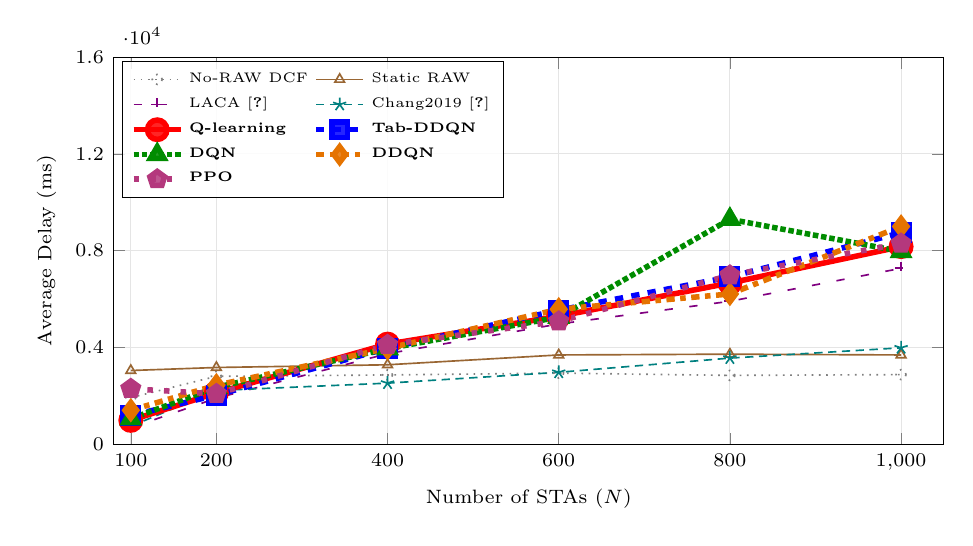
\begin{tikzpicture}
\begin{axis}[
  width=\columnwidth, height=6.5cm,
  xlabel={Number of STAs ($N$)},
  ylabel={Average Delay (ms)},
  xmin=80, xmax=1050,
  ymin=0, ymax=16000,
  xtick={100,200,400,600,800,1000},
  ytick={0,4000,8000,12000,16000},
  legend style={font=\tiny, cells={anchor=west}, legend columns=2,
                at={(0.01,0.99)}, anchor=north west, draw=black,
                fill=white, fill opacity=0.85, text opacity=1},
  grid=both, grid style={gray!20},
  tick label style={font=\scriptsize},
  label style={font=\scriptsize},
]
% ---- Baselines ----
\addplot[color=gray,          line width=0.6pt, dotted,
         mark=o,        mark size=1.8pt] coordinates {
  (100,1930)(200,2812)(400,2869)(600,2945)(800,2850)(1000,2883)
}; \addlegendentry{No-RAW DCF}
\addplot[color=brown!80!black, line width=0.6pt, solid,
         mark=triangle,  mark size=2pt] coordinates {
  (100,3052)(200,3177)(400,3289)(600,3695)(800,3727)(1000,3695)
}; \addlegendentry{Static RAW}
\addplot[color=violet,         line width=0.6pt, loosely dashed,
         mark=+,         mark size=2.2pt] coordinates {
  (100,687)(200,1909)(400,3749)(600,4974)(800,5912)(1000,7274)
}; \addlegendentry{LACA~\cite{taramit2023laca}}
\addplot[color=teal,           line width=0.6pt, densely dashed,
         mark=star,      mark size=2.5pt] coordinates {
  (100,747)(200,2226)(400,2530)(600,2978)(800,3565)(1000,3990)
}; \addlegendentry{Chang2019~\cite{chang2019traffic}}
% ---- RL variants ----
\addplot[color=red,                   line width=2pt, solid,
         mark=*,         mark size=3.5pt,
         mark options={solid,fill=red}] coordinates {
  (100,992)(200,2130)(400,4143)(600,5293)(800,6668)(1000,8171)
}; \addlegendentry{\textbf{Q-learning}}
\addplot[color=blue,                  line width=2pt, dashed,
         mark=square*,   mark size=2.8pt,
         mark options={solid,fill=blue}] coordinates {
  (100,1192)(200,2035)(400,3969)(600,5545)(800,6918)(1000,8744)
}; \addlegendentry{\textbf{Tab-DDQN}}
\addplot[color=green!55!black,        line width=2pt, densely dotted,
         mark=triangle*,  mark size=2.8pt,
         mark options={solid,fill=green!55!black}] coordinates {
  (100,1058)(200,2360)(400,3955)(600,5257)(800,9300)(1000,7971)
}; \addlegendentry{\textbf{DQN}}
\addplot[color=orange!90!black,       line width=2pt, dashdotted,
         mark=diamond*,   mark size=2.8pt,
         mark options={solid,fill=orange!90!black}] coordinates {
  (100,1411)(200,2445)(400,3969)(600,5583)(800,6214)(1000,9003)
}; \addlegendentry{\textbf{DDQN}}
\addplot[color=magenta!70!black,      line width=2pt, loosely dotted,
         mark=pentagon*,  mark size=2.8pt,
         mark options={solid,fill=magenta!70!black}] coordinates {
  (100,2298)(200,2087)(400,4114)(600,5083)(800,6986)(1000,8300)
}; \addlegendentry{\textbf{PPO}}
\end{axis}
\end{tikzpicture}
\caption{Average end-to-end delay (multi-episode-trained RL).  RL delay is
  close to LACA at $N\!=\!200$ (within $7\,\%$, Tab-DDQN) but PPO's delay at
  $N\!=\!100$ is $3.3\times$ LACA's, mirroring its low PDR there.  RL delay
  grows to $2.8$--$3.1\times$ No-RAW's value at $N\!=\!1000$.  Tabular
  Q-learning is the most competitive RL variant at $N\!=\!100$; PPO is least
  penalised at $N\!=\!600$; DDQN at $N\!=\!800$; DQN at $N\!=\!1000$.
  Chang2019 records the lowest delay of all nine policies at $N\!=\!400$
  (2530\,ms), a side-effect of its sharply collapsed PDR at that density.
  RL lines: 2\,pt; baseline lines: 0.6\,pt.}
\label{fig:delay}
\end{figure}

\subsection{Energy Consumption and Efficiency}

Table~\ref{tab:energy} reports per-STA energy at $N = 200$.
Compared to no-RAW (2559\,mJ), all RAW-enabled policies reduce per-STA
total energy by $3.96$--$6.3\times$ (406--646\,mJ), because STAs sleep
outside their assigned RAW slots while idle power dominates in the
no-RAW case.
Chang2019 sits at the high end of this range (646\,mJ): its grouping at
$N=200$ already spans most of the AID space with comparatively wide RAW
slots, so each STA's idle (contention) window is larger than under the
other RAW-enabled policies, even though its PDR (0.434) is far below LACA's
and every RL variant's.

Two observations from the breakdown are noteworthy.
\textbf{(i)~PPO offers the best PDR-per-energy trade-off at $N=200$ among
all nine policies}: it delivers PDR $=0.949$ at 460\,mJ, i.e.\ $+0.9$\,pp
higher PDR than LACA (0.940 at 533\,mJ) for $14\,\%$ \emph{less} energy —
the trained RL controller both beats and is cheaper than the strongest
baseline.
The other RL variants (tabular, Tab-DDQN, DQN, DDQN) fall in the
406--463\,mJ band with PDR between 0.85 and 0.94, all comparable to or
better than LACA's energy budget; DDQN has the lowest total energy of any
RAW-enabled policy (406\,mJ) but also the lowest PDR among RL variants at
this density (0.846).
\textbf{(ii)~Sleep energy is similar ($\approx48$–$54$\,mJ) across all
RAW-enabled policies} (static, LACA, Chang2019, and all five RL variants),
confirming that the sleep-time mechanism is equally effective regardless
of the scheduling algorithm, and that the dominant energy difference across
policies lies in idle (contention) time rather than in transmit/receive or
sleep energy.
The DATA frame airtime at MCS0 with 128-byte payload is
$T_\text{data}=t_\text{preamble}+t_\text{header}+(128\!\times\!8)/150\,\text{kbps}
\approx 0.40+6.83=7.23$\,ms,
so one retransmitted DATA frame costs
$P_\text{tx}\!\times\!T_\text{data}=180\,\text{mW}\!\times\!7.23\,\text{ms}
\approx 1.30$\,mJ in TX energy, and with the contention window doubled
after the first failure
($\bar{t}_\text{bo}^{\prime}=\tfrac{CW_\text{min}}{2}\sigma
\approx 15\!\times\!52\,\mu\text{s}=780\,\mu\text{s}$),
the additional idle backoff penalty is
$P_\text{idle}\!\times\!780\,\mu\text{s}\approx0.016$\,mJ,
giving a total per-retry cost of $\approx1.32$\,mJ — negligible relative to
the 427--533\,mJ totals.
The dominant energy cost per successfully delivered packet is one complete
DATA–ACK exchange:
$P_\text{tx}\!\times\!T_\text{data} + P_\text{rx}\!\times\!T_\text{ACK}
+ P_\text{idle}\!\times\!(\bar{t}_\text{bo}+T_\text{DIFS})
\approx 1.30+0.07+0.02=1.39$\,mJ.

Fig.~\ref{fig:ee} shows energy efficiency (useful throughput per joule).
At $N = 100$, Tab-DDQN achieves the highest EE of all nine policies
(61.8\,kbit/J), $+12.5\,\%$ above LACA (54.9); Chang2019 reaches 58.4, the
third-highest value overall (behind Tab-DDQN and DQN's 58.7) and above
LACA, reflecting its PDR$=1.000$ at this density.
At $N = 200$, DDQN leads (51.3), $+18.6\,\%$ above LACA (43.3); Chang2019's
EE collapses to 16.5 at this density — below every other policy except
No-RAW (2.35) — as a direct consequence of its PDR collapse to 0.434.
At $N \in \{400,600,800,1000\}$, PPO leads (34.0, 24.8, 15.0, 10.1),
$+73.1\,\%$, $+96.0\,\%$, $+75.8\,\%$, and $+68.1\,\%$ above the best
baseline (LACA at $N=400$, static RAW at $N\in\{600,800,1000\}$).
Chang2019's EE continues to decline (4.9, 3.0, 1.9, 1.4 at
$N\in\{400,600,800,1000\}$) — consistently above No-RAW but below Static
RAW, LACA, and every RL variant — tracking its low and falling PDR at these
densities.
An RL variant therefore achieves the highest EE at every density level,
with the margin over the best baseline now substantially larger than under
single-episode training — particularly at $N \in \{400,600,800,1000\}$,
where multi-episode-trained RL is $68$--$96\,\%$ more efficient than the
best baseline, compared to $4$--$21\,\%$ before training.
The efficiency gain has two sources: (i)~higher PDR means more bits
delivered per joule; (ii)~phase partitioning widens per-slot windows,
reducing the fraction of each beacon interval wasted on failed contention
cycles.

\begin{table}[t]
\centering
\caption{Per-STA Energy Breakdown at $N = 200$ (mean over 3 seeds),
multi-episode-trained RL.
Bold marks the lowest idle energy among RAW-enabled policies.
TX+RX is the residual (Total $-$ Idle $-$ Sleep).
All values include the association-phase idle overhead
(64–72\,mJ for RAW policies; 215\,mJ for No-RAW — see Table~\ref{tab:assoc}).}
\label{tab:energy}
\setlength{\tabcolsep}{4pt}
\begin{tabular}{lrrrrr}
\toprule
Policy & Total & Idle & Sleep & TX+RX & PDR \\
       & (mJ)  & (mJ) & (mJ) & (mJ) & \\
\midrule
No-RAW          & 2559 & 2356 &  0.0 & 203 & 0.245 \\
Static RAW      &  443 &  243 & 53.0 & 147 & 0.472 \\
LACA            &  533 &  311 & 51.2 & 171 & 0.940 \\
Chang2019       &  646 &  422 & 48.4 & 176 & 0.434 \\
\midrule
Tabular         &  460 &  245 & 52.9 & 162 & 0.903 \\
Tab-DDQN        &  455 &  233 & 53.2 & 169 & 0.921 \\
DQN             &  463 &  251 & 52.7 & 160 & 0.937 \\
\textbf{DDQN}   &  406 & \textbf{192} & 54.2 & 160 & 0.846 \\
PPO             &  460 &  247 & 52.8 & 161 & \textbf{0.949} \\
\bottomrule
\end{tabular}
\end{table}

\begin{figure}[t]
\centering
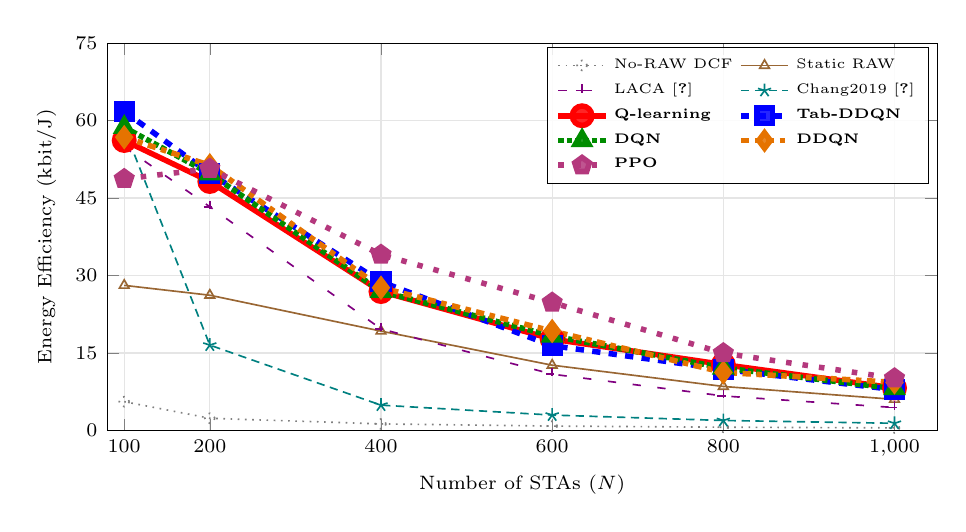
\begin{tikzpicture}
\begin{axis}[
  width=\columnwidth, height=6.5cm,
  xlabel={Number of STAs ($N$)},
  ylabel={Energy Efficiency (kbit/J)},
  xmin=80, xmax=1050,
  ymin=0, ymax=75,
  xtick={100,200,400,600,800,1000},
  ytick={0,15,30,45,60,75},
  legend style={font=\tiny, cells={anchor=west}, legend columns=2,
                at={(0.99,0.99)}, anchor=north east, draw=black,
                fill=white, fill opacity=0.85, text opacity=1},
  grid=both, grid style={gray!20},
  tick label style={font=\scriptsize},
  label style={font=\scriptsize},
]
% ---- Baselines ----
\addplot[color=gray,           line width=0.6pt, dotted,
         mark=o,        mark size=1.8pt] coordinates {
  (100,5.57)(200,2.35)(400,1.26)(600,0.84)(800,0.62)(1000,0.49)
}; \addlegendentry{No-RAW DCF}
\addplot[color=brown!80!black,  line width=0.6pt, solid,
         mark=triangle,  mark size=2pt] coordinates {
  (100,28.09)(200,26.18)(400,19.23)(600,12.63)(800,8.51)(1000,6.01)
}; \addlegendentry{Static RAW}
\addplot[color=violet,          line width=0.6pt, loosely dashed,
         mark=+,         mark size=2.2pt] coordinates {
  (100,54.91)(200,43.31)(400,19.66)(600,10.89)(800,6.67)(1000,4.43)
}; \addlegendentry{LACA~\cite{taramit2023laca}}
\addplot[color=teal,            line width=0.6pt, densely dashed,
         mark=star,       mark size=2.5pt] coordinates {
  (100,58.40)(200,16.52)(400,4.89)(600,2.97)(800,1.92)(1000,1.38)
}; \addlegendentry{Chang2019~\cite{chang2019traffic}}
% ---- RL variants ----
\addplot[color=red,                    line width=2pt, solid,
         mark=*,         mark size=3.5pt,
         mark options={solid,fill=red}] coordinates {
  (100,56.15)(200,48.21)(400,26.90)(600,17.69)(800,12.75)(1000,8.22)
}; \addlegendentry{\textbf{Q-learning}}
\addplot[color=blue,                   line width=2pt, dashed,
         mark=square*,   mark size=2.8pt,
         mark options={solid,fill=blue}] coordinates {
  (100,61.76)(200,49.77)(400,28.78)(600,16.41)(800,11.83)(1000,7.90)
}; \addlegendentry{\textbf{Tab-DDQN}}
\addplot[color=green!55!black,         line width=2pt, densely dotted,
         mark=triangle*,  mark size=2.8pt,
         mark options={solid,fill=green!55!black}] coordinates {
  (100,58.70)(200,49.72)(400,26.93)(600,18.30)(800,12.11)(1000,8.11)
}; \addlegendentry{\textbf{DQN}}
\addplot[color=orange!90!black,        line width=2pt, dashdotted,
         mark=diamond*,   mark size=2.8pt,
         mark options={solid,fill=orange!90!black}] coordinates {
  (100,56.78)(200,51.34)(400,27.63)(600,19.24)(800,11.23)(1000,9.31)
}; \addlegendentry{\textbf{DDQN}}
\addplot[color=magenta!70!black,       line width=2pt, loosely dotted,
         mark=pentagon*,  mark size=2.8pt,
         mark options={solid,fill=magenta!70!black}] coordinates {
  (100,48.70)(200,50.68)(400,34.03)(600,24.76)(800,14.96)(1000,10.10)
}; \addlegendentry{\textbf{PPO}}
\end{axis}
\end{tikzpicture}
\caption{Energy efficiency (kbit/J) — five multi-episode-trained RL
  variants and four baselines.  An RL variant achieves the highest EE at
  every $N$: Tab-DDQN at $N\!=\!100$, DDQN at $N\!=\!200$, and PPO at
  $N\!\in\!\{400,600,800,1000\}$, with margins of
  $13$--$96\,\%$ over the best baseline.  Chang2019 is competitive at
  $N\!=\!100$ (third-highest overall) but collapses for $N\!\geq\!200$.}
\label{fig:ee}
\end{figure}

\subsection{Training Convergence}
\label{sec:training}

All results in this section use the multi-episode, convergence-based
training procedure of Sec.~\ref{sec:setup}, applied independently to each
of the 30 (architecture, $N$) pairs.
Across the sweep, the number of training episodes required ranges from 4
to the 20-episode cap, with a mean of $11.3$ episodes.
Three combinations converge in the minimum 4 episodes (DDQN at $N=100$, DQN
at $N=1000$, Tab-DDQN at $N=800$), while six combinations exhaust the full
20-episode budget without satisfying the convergence criterion (Tab-DDQN at
$N=200$; DQN at $N\in\{200,400\}$; DDQN at $N\in\{200,600\}$; PPO at
$N=100$).
No clear relationship emerges between convergence speed and final PDR: PPO
at $N=100$ requires the full 20 episodes yet attains the \emph{lowest}
evaluation PDR of any RL variant at that density (0.863), while DDQN at
$N=100$ converges in just 4 episodes and attains a solid evaluation PDR
(0.969).
This indicates that PDR variance across training seeds — rather than a
monotonic learning curve — is the dominant factor triggering early
stopping, particularly at low-to-moderate density where individual episodes
are short (235 beacon steps) and per-episode PDR is sensitive to the
specific traffic/contention realisation of each training seed.
The remainder of this section reports results from the resulting 30 trained
checkpoints, evaluated on three held-out seeds disjoint from training.

\subsection{RL Algorithm Variant Comparison}

Figs.~\ref{fig:pdr}--\ref{fig:ee} show all five multi-episode-trained RL
variants alongside the four baselines.
Table~\ref{tab:rl_pdr} lists the 95\,\% CI half-widths.
Four findings stand out.

\textbf{(i)~Stability is density-dependent rather than algorithm-dependent.}
At $N=100$, DQN is tightest (CI $\pm0.015$), with tabular close behind
($\pm0.024$) and Tab-DDQN moderate ($\pm0.033$); DDQN is wider ($\pm0.080$)
and PPO is by far the widest ($\pm0.137$), reflecting its poor and variable
performance at this density.
At $N=200$ — the transition region — DDQN is widest ($\pm0.133$), with
tabular and DQN both around $\pm0.110$, while Tab-DDQN is tightest
($\pm0.032$) and PPO close behind ($\pm0.047$) despite achieving the highest
mean PDR.
For $N\geq600$, PPO is consistently among the tightest ($\pm0.009$,
$\pm0.012$, $\pm0.050$ at $N=600,800,1000$) even though it leads PDR at all
three densities, while Tab-DDQN is repeatedly among the widest ($\pm0.109$,
$\pm0.044$, $\pm0.069$).

\textbf{(ii)~PPO dominates PDR at every density except $N=100$.}
PPO leads at $N\in\{200,400,600,800,1000\}$ (0.949, 0.566, 0.417, 0.281,
0.210), exceeding the best baseline by $+0.9$, $+18.3$, $+15.5$, $+9.1$, and
$+6.3$\,pp respectively.
At $N=100$, PPO is instead the \emph{weakest} RL variant by a wide margin
(0.863); DQN is the strongest RL controller there (0.993) but, alone among
all densities, does not surpass the best baseline (LACA, 1.000).
Tabular Q-learning, Tab-DDQN, DQN, and DDQN never lead any density, though
all four still exceed the best baseline at $N\in\{400,600,800,1000\}$.

\textbf{(iii)~Energy efficiency mirrors the PDR leader at most densities,
but not at $N=100$.}
Tab-DDQN gives the best EE at $N=100$ (61.8\,kbit/J, $+12.5\,\%$ over LACA)
despite PPO's poor PDR there; DDQN leads at $N=200$ (51.3, $+18.6\,\%$ over
LACA); and PPO leads at $N\in\{400,600,800,1000\}$ (34.0, 24.8, 15.0, 10.1,
i.e.\ $+73.1$, $+96.0$, $+75.8$, and $+68.1\,\%$ over the best baseline).
The EE margins under multi-episode training ($68$--$96\,\%$ at
$N\geq400$) are substantially larger than the $4$--$21\,\%$ margins observed
with single-episode training, because the PDR gains compound directly into
useful bits delivered per joule while idle/sleep energy is largely
policy-independent (Table~\ref{tab:energy}).

\textbf{(iv)~The delay-optimal RL variant shifts with $N$, but the
multi-episode-trained variants are markedly closer to the baselines than
their single-episode counterparts — except PPO at $N=100$.}
Tabular Q-learning has the lowest RL delay at $N=100$ (992\,ms, $45\,\%$
above LACA); Tab-DDQN at $N=200$ (2035\,ms, only $7\,\%$ above LACA); DQN at
$N\in\{400,1000\}$ (3955, 7971\,ms); PPO at $N=600$ (5083\,ms); and DDQN at
$N=800$ (6214\,ms).
PPO's delay at $N=100$ (2298\,ms, $3.3\times$ LACA's) is the only extreme
outlier among the multi-episode-trained variants, consistent with its
anomalously low PDR at that density; at $N=1000$ the spread across RL
variants is modest (7971--9003\,ms, a $13\,\%$ range).

\textbf{Recommendation.}
Across the full win-count tally over all evaluated metrics (42 chances: 7
metrics $\times$ 6 densities, ties counted for every tied policy), PPO
dominates with 28 wins, far ahead of LACA (7), No-RAW (4) and Chang2019 (4,
both mostly delay artefacts of near-zero PDR), Tab-DDQN (1), and DDQN (1);
tabular Q-learning, DQN, and static RAW win 0.
Chang2019's four wins are concentrated at $N=100$, where it ties LACA on
PDR, throughput, and fairness (each $=1.000$/$20.48$\,kb/s), plus a single
delay win at $N=400$ where its collapsed PDR drops most traffic before it
accrues queuing delay.
For $N=100$, LACA and Chang2019 are jointly the best overall choice
(PDR $=1.000$), with DQN the closest RL approximation (PDR 0.993, delay
$54\,\%$ above LACA); PPO should be avoided at this density given its poor
PDR (0.863) and high delay (2298\,ms).
For $N\geq200$, Chang2019 is not competitive — its PDR falls below 0.45 and
keeps declining, so it is recommended only at $N=100$.
For $N\in\{200,400,600,800,1000\}$, PPO is recommended without
qualification: it gives the best PDR at every one of these densities, and
the best EE at $N\in\{400,600,800,1000\}$.
Tabular Q-learning, Tab-DDQN, DQN, and DDQN, while no longer competitive on
PDR against PPO at $N\geq200$, still exceed the best baseline's PDR at
$N\geq400$ and remain viable lower-complexity fallbacks; DDQN in particular
offers competitive EE at $N\in\{100,200,1000\}$ and Tab-DDQN at $N=100$.

\begin{table}[t]
\centering
\caption{Multi-episode-trained PDR: mean $\pm$ 95\,\%~CI half-width.
  Bold marks the best RL variant per row.
  PPO leads at $N\in\{200,400,600,800,1000\}$; DQN at $N=100$.}
\label{tab:rl_pdr}
\setlength{\tabcolsep}{3pt}
{\scriptsize
\begin{tabular}{r ccccc}
\toprule
$N$ & Q-learn & Tab-DDQN & DQN & DDQN & PPO \\
\midrule
100  & 0.989{\tiny$\pm$0.024} & 0.988{\tiny$\pm$0.033} & \textbf{0.993{\tiny$\pm$0.015}} & 0.969{\tiny$\pm$0.080} & 0.863{\tiny$\pm$0.137} \\
200  & 0.904{\tiny$\pm$0.110} & 0.921{\tiny$\pm$0.032} & 0.937{\tiny$\pm$0.110} & 0.846{\tiny$\pm$0.133} & \textbf{0.949{\tiny$\pm$0.047}} \\
400  & 0.479{\tiny$\pm$0.094} & 0.511{\tiny$\pm$0.061} & 0.458{\tiny$\pm$0.096} & 0.496{\tiny$\pm$0.037} & \textbf{0.566{\tiny$\pm$0.020}} \\
600  & 0.323{\tiny$\pm$0.040} & 0.296{\tiny$\pm$0.109} & 0.337{\tiny$\pm$0.008} & 0.340{\tiny$\pm$0.037} & \textbf{0.417{\tiny$\pm$0.009}} \\
800  & 0.251{\tiny$\pm$0.026} & 0.235{\tiny$\pm$0.044} & 0.221{\tiny$\pm$0.077} & 0.224{\tiny$\pm$0.072} & \textbf{0.281{\tiny$\pm$0.012}} \\
1000  & 0.181{\tiny$\pm$0.023} & 0.170{\tiny$\pm$0.069} & 0.180{\tiny$\pm$0.025} & 0.196{\tiny$\pm$0.004} & \textbf{0.210{\tiny$\pm$0.050}} \\
\bottomrule
\end{tabular}
}
\end{table}

\section{Conclusion}

This paper proposes RL-RAW (v8), an autonomous tabular Q-learning policy
for IEEE~802.11ah RAW scheduling that jointly tunes group count, slot count,
slot duration, and — crucially — beacon phase count, all from AP-side MAC
statistics without per-STA feedback, pre-computed tables, or any hardcoded
station-count threshold.
Three key design elements distinguish RL-RAW from prior heuristic approaches:
(i)~two new Q-learning actions (\textsc{PhasesInc}/\textsc{PhasesDec}) that
let the agent discover the right AID-space partitioning for \emph{any} $N$
from the reward signal alone, starting from $P = 1$;
(ii)~an eight-dimensional state space that includes MAC retry-rate and
phase-count buckets as explicit signals for within-slot and
inter-beacon delay, enabling Q-learning to distinguish both contention
and scheduling pressure; and
(iii)~a six-term delay-aware reward that penalises retry accumulation,
phase-cycling wait, and slot inadequacy alongside PDR, collisions,
and RAW overhead.
Each of five RL controller architectures was trained with a
\emph{multi-episode, convergence-based} procedure (3--20 episodes per
architecture/$N$ pair, stopping once consecutive-episode PDR change falls
below $0.01$), then evaluated against four baselines (No-RAW, Static RAW,
LACA, and Chang2019~\cite{chang2019traffic}, a regression-based
traffic-aware grouping scheme re-implemented as an additional benchmark)
across $N \in \{100, \ldots, 1000\}$ with a corrected implementation
featuring consistent action masking on all selection paths and masked
Bellman targets.
Multi-episode training qualitatively changes the competitive picture
relative to a single training episode.
At $N=100$, LACA and Chang2019 jointly attain the strongest PDR overall
($=1.000$), with trained DQN closest ($0.993$, delay $54\,\%$ above LACA)
— the only density at which no RL variant surpasses the best baseline.
Notably, PPO is the \emph{weakest} RL variant at this density ($0.863$,
delay $3.3\times$ LACA's).
Chang2019's strong showing at $N=100$ does not generalise: its PDR
collapses to $0.434$ at $N=200$ and falls further to $0.065$ by $N=1000$,
though it incidentally records the lowest end-to-end delay of all nine
policies at $N=400$ (2530\,ms) as a side-effect of dropping most traffic
before it queues.
From $N=200$ onward, PPO exceeds \emph{every} baseline at \emph{every}
density: $0.949$, $0.566$, $0.417$, $0.281$, and $0.210$ at
$N\in\{200,400,600,800,1000\}$ — $+0.9$, $+18.3$, $+15.5$, $+9.1$, and
$+6.3$\,pp over the best baseline respectively.
Energy efficiency improves correspondingly — an RL variant achieves the
highest kbit/J at every density (Tab-DDQN at $N=100$, DDQN at $N=200$, PPO
at $N\in\{400,600,800,1000\}$), with margins of $13$--$96\,\%$ over
the best baseline, substantially larger than the
$4$--$21\,\%$ margins observed with single-episode training.
At $N=200$, PPO simultaneously beats LACA on PDR \emph{and} uses $14\,\%$
less per-STA energy (460 vs.\ 533\,mJ), demonstrating that the trained
controller is not merely competitive but Pareto-superior to the strongest
baseline at that density.
An energy analysis reveals that data-retransmission overhead is negligible
relative to the 406--533\,mJ per-STA totals at $N=200$, and that sleep
energy ($\approx51$--$54$\,mJ) is essentially policy-independent — the
dominant cross-policy difference is idle (contention) energy.
The cost of these PDR/EE gains remains delay: at $N\geq400$, the best RL
delay is $20$--$116\,\%$ higher than static RAW, growing with $N$, though
multi-episode-trained variants (other than PPO at $N=100$) avoid the extreme
single-episode delay spikes (e.g.\ DDQN previously reached $14\,730$\,ms at
$N=1000$; the worst multi-episode RL delay at $N=1000$ is $9003$\,ms).
Across the full win-count tally (42 chances), PPO dominates with 28 wins —
far ahead of LACA (7), No-RAW (4) and Chang2019 (4, both mostly delay
artefacts of near-zero PDR), Tab-DDQN (1), and DDQN (1); tabular
Q-learning, DQN, and static RAW win nothing.
PPO is therefore the recommended controller for $N\in\{200,400,600,800,1000\}$,
where it leads PDR at every density and EE at $N\in\{400,600,800,1000\}$.
At $N=100$, LACA remains the overall best choice, with trained DQN the
closest RL approximation; PPO should be avoided at this density.
In future work, we will extend RL-RAW to heterogeneous traffic, multi-rate
PHY environments, and multi-AP coordination, and investigate why PPO's
training dynamics at $N=100$ converge to a markedly weaker policy than at
every other density.

% -----------------------------------------------------------------------
\balance
\begin{thebibliography}{15}

\bibitem{std80211ah}
\textit{IEEE Standard 802.11ah-2016}: Wireless LAN MAC and PHY
Specifications Amendment 2: Sub 1\,GHz Operation, IEEE, 2016.

\bibitem{tian2021survey}
L.~Tian, S.~Santi, A.~Seferagi\'{c}, J.~Lan, and J.~Famaey,
``Wi-Fi HaLow for the Internet of Things: An up-to-date survey on
IEEE~802.11ah research,''
\textit{J. Netw. Comput. Appl.}, vol.~182, p.~103036, 2021.

\bibitem{ahmed2021mac}
N.~Ahmed, D.~De, F.~A.~Barbhuiya, and M.~I.~Hussain,
``MAC protocols for IEEE~802.11ah-based Internet of Things: A survey,''
\textit{IEEE IoT J.}, vol.~9, no.~2, pp.~916--938, 2022.

\bibitem{tian2016taroa}
L.~Tian, J.~Famaey, and S.~Latr\'{e},
``Evaluation of the IEEE~802.11ah restricted access window mechanism
for dense IoT networks,''
in \textit{Proc.\ IEEE WoWMoM}, 2016, pp.~1--9.

\bibitem{tian2017etaroa}
L.~Tian, S.~Santi, S.~Latr\'{e}, and J.~Famaey,
``Accurate sensor traffic estimation for station grouping in highly
dense IEEE~802.11ah networks,''
in \textit{Proc.\ ACM EWSN Workshop}, 2017, pp.~1--9.

\bibitem{liu2020roraw}
Z.~Liu and P.~Lv,
``RO-RAW: Run-time restricted access window optimization in
IEEE~802.11ah with extended Kalman filter,''
\textit{Wireless Commun. Mobile Comput.}, vol.~2020, p.~8876669, 2020.

\bibitem{chang2019traffic}
T.-C.~Chang, C.-H.~Lin, K.~C.-J.~Lin, and W.-T.~Chen,
``Traffic-aware sensor grouping for IEEE~802.11ah networks: Regression
based analysis and design,''
\textit{IEEE Trans. Mobile Comput.}, vol.~18, no.~3, pp.~674--687, 2019.

\bibitem{hasi2022}
M.~A.~A.~Hasi, M.~D.~Haque, and M.~A.~Siddik,
``Traffic demand-based grouping for fairness among the RAW groups of
heterogeneous stations in IEEE~802.11ah IoT networks,''
in \textit{Proc.\ ICAEEE}, IEEE, 2022, pp.~1--6.

\bibitem{taramit2023laca}
H.~Taramit, L.~Orozco-Barbosa, A.~Haqiq, J.~J.~C.~Escoto, and J.~Gomez,
``Load-aware channel allocation for IEEE~802.11ah-based networks,''
\textit{IEEE Access}, vol.~11, pp.~24\,484--24\,496, 2023.

\bibitem{nandhini2025}
R.~Nandhini and R.~Radha,
``Neuro-fuzzy ARX approach for dynamic RAW duration adaptation in
event triggered large scale IEEE~802.11ah networks,''
\textit{IEEE Access}, vol.~13, pp.~162\,588--162\,610, 2025.

\bibitem{watkins1992}
C.~J.~C.~H.~Watkins and P.~Dayan,
``Q-learning,''
\textit{Mach. Learn.}, vol.~8, no.~3--4, pp.~279--292, 1992.

\bibitem{mnih2015}
V.~Mnih \textit{et al.},
``Human-level control through deep reinforcement learning,''
\textit{Nature}, vol.~518, pp.~529--533, 2015.

\bibitem{sutton2018}
R.~S.~Sutton and A.~G.~Barto,
\textit{Reinforcement Learning: An Introduction}, 2nd~ed.
MIT Press, 2018.

\bibitem{hasselt2010}
H.~van Hasselt,
``Double Q-learning,''
in \textit{Proc.\ NeurIPS}, 2010, pp.~2613--2621.

\bibitem{vanhasselt2016}
H.~van Hasselt, A.~Guez, and D.~Silver,
``Deep reinforcement learning with double Q-learning,''
in \textit{Proc.\ AAAI}, 2016, pp.~2094--2100.

\bibitem{schulman2015}
J.~Schulman, P.~Moritz, S.~Levine, M.~Jordan, and P.~Abbeel,
``High-dimensional continuous control using generalized advantage
estimation,''
in \textit{Proc.\ ICLR}, 2016.

\end{thebibliography}

\end{document}
